\documentclass{beamer}
\usetheme{Copenhagen}
\usecolortheme{crane}
\usepackage[utf8]{inputenc}
\usefonttheme{structuresmallcapsserif}
\usepackage{lmodern, kotex, babel, graphicx, cancel}
\usepackage[showdow]{datetime2}

\newcommand*{\datefmt}[3]{%
  \number#3~\pgfcalendarmonthname{#2} \number#1%
}

\title{Workbook Examples \\ Chapter $4$ \\ Math $1100$}
\author{Don D. Kim}
%\institute{\Large{\textsc{University of Missouri}}}
\date{\datefmt{\year}{\month}{\day}}

\titlegraphic{\vfill \centering 
\includegraphics[scale=1.0]{Mizzou.png}\vfill}

\begin {document}

\begin{frame}
	\titlepage
\end{frame}

\begin{frame}
	\frametitle{Outline}
	\tableofcontents
\end{frame}

\section{$\S 4.1$: Polynomial Functions and Models}

\begin{frame}
	\frametitle{Objectives}
	\begin{enumerate}
		\item[]<1-> Determine the behavior of the graph of a polynomial function using the leading term test.
		\item[]<2->Factor polynomial functions, and find the zeros and their multiplicities.
	\end{enumerate}
\end{frame}

\begin{frame}
	\frametitle{Polynomial Function}
	\begin{enumerate}
		\item[]<1-> A \emph{polynomial function} $P$ is given by
		\item[]<2->
		\[
			P(x)=a_{n}x^{n}+a_{n-1}x^{n-1}+\dots+a_{1}x+a_{0},
		\]
		\item[]<3->where the coefficients $a_{n}, a_{n-1}, \dots, a_{1}, a_{0}$ are real numbers and the exponents are whole numbers.
	\end{enumerate}
\end{frame}

\begin{frame}
	\frametitle{Example}
	\begin{enumerate}
		\item[]<1->Determine the leading term, the leading coefficient, and the degree of the polynomial.  Then classify the polynomial as a constant, linear, quadratic, cubic or quartic.
		\item[]<2->
		\[
			g(x)=-\frac{1}{6}x^{3}-4x+8.
		\]
		\item[]<3-> \textsc{Solution:}
		\item[]<4-> The leading term, i.e. the term with the highest degree, is
		\item[]<5-> \[ \frac{1}{6}x^{3}. \]
		\item[]<6->The degree of $g(x)$ is $3$.
		\item[]<7->The polynomial is a cubic polynomial.
	\end{enumerate}
\end{frame}

\begin{frame}
	\frametitle{Example}
	\begin{enumerate}
		\item[]<1->Determine the leading term, the leading coefficient, and the degree of the polynomial.  Then classify the polynomial as a constant, linear, quadratic, cubic or quartic.
		\item[]<2->
		\[
			g(x)=2.4x^{4}+5x^{2}-x+\frac{5}{8}.
		\]
		\item[]<3-> \textsc{Solution:}
		\item[]<4-> The leading term, i.e. the term with the highest degree, is
		\item[]<5-> \[ 2.4x^{4}. \]
		\item[]<6->The degree of $g(x)$ is $4$.
		\item[]<7->The polynomial is a quartic polynomial.
	\end{enumerate}
\end{frame}

\begin{frame}
	\frametitle{Example}
	\begin{enumerate}
		\item[]<1->Determine the leading term, the leading coefficient, and the degree of the polynomial.  Then classify the polynomial as a constant, linear, quadratic, cubic or quartic.
		\item[]<2->
		\[
			g(x)=-3x+7x^{2}+x^{3}.
		\]
		\item[]<3-> \textsc{Solution:}
		\item[]<4-> The leading term, i.e. the term with the highest degree, is
		\item[]<5-> \[ x^{3}. \]
		\item[]<6->The degree of $g(x)$ is $3$.
		\item[]<7->The polynomial is a cubic polynomial.
	\end{enumerate}
\end{frame}

\begin{frame}
	\frametitle{Example}
	\begin{enumerate}
		\item[]<1->Determine the leading term, the leading coefficient, and the degree of the polynomial.  Then classify the polynomial as a constant, linear, quadratic, cubic or quartic.
		\item[]<2->
		\[
			g(x)=-4x^{2}+9x^{4}+x^{3}.
		\]
		\item[]<3-> \textsc{Solution:}
		\item[]<4-> The leading term, i.e. the term with the highest degree, is
		\item[]<5-> \[ 9x^{4}. \]
		\item[]<6->The degree of $g(x)$ is $4$.
		\item[]<7->The polynomial is a quartic polynomial.
	\end{enumerate}
\end{frame}

\begin{frame}
	\frametitle{Example}
	\begin{enumerate}
		\item[]<1-> Given
		\[
			f(x)=x^{2}-2x-3=(x+1)(x-3),
		\]
		\item[]<2->
		\begin{figure}
			\begin{center}
				\caption{$f(x)=x^{2}-2x-3$}
				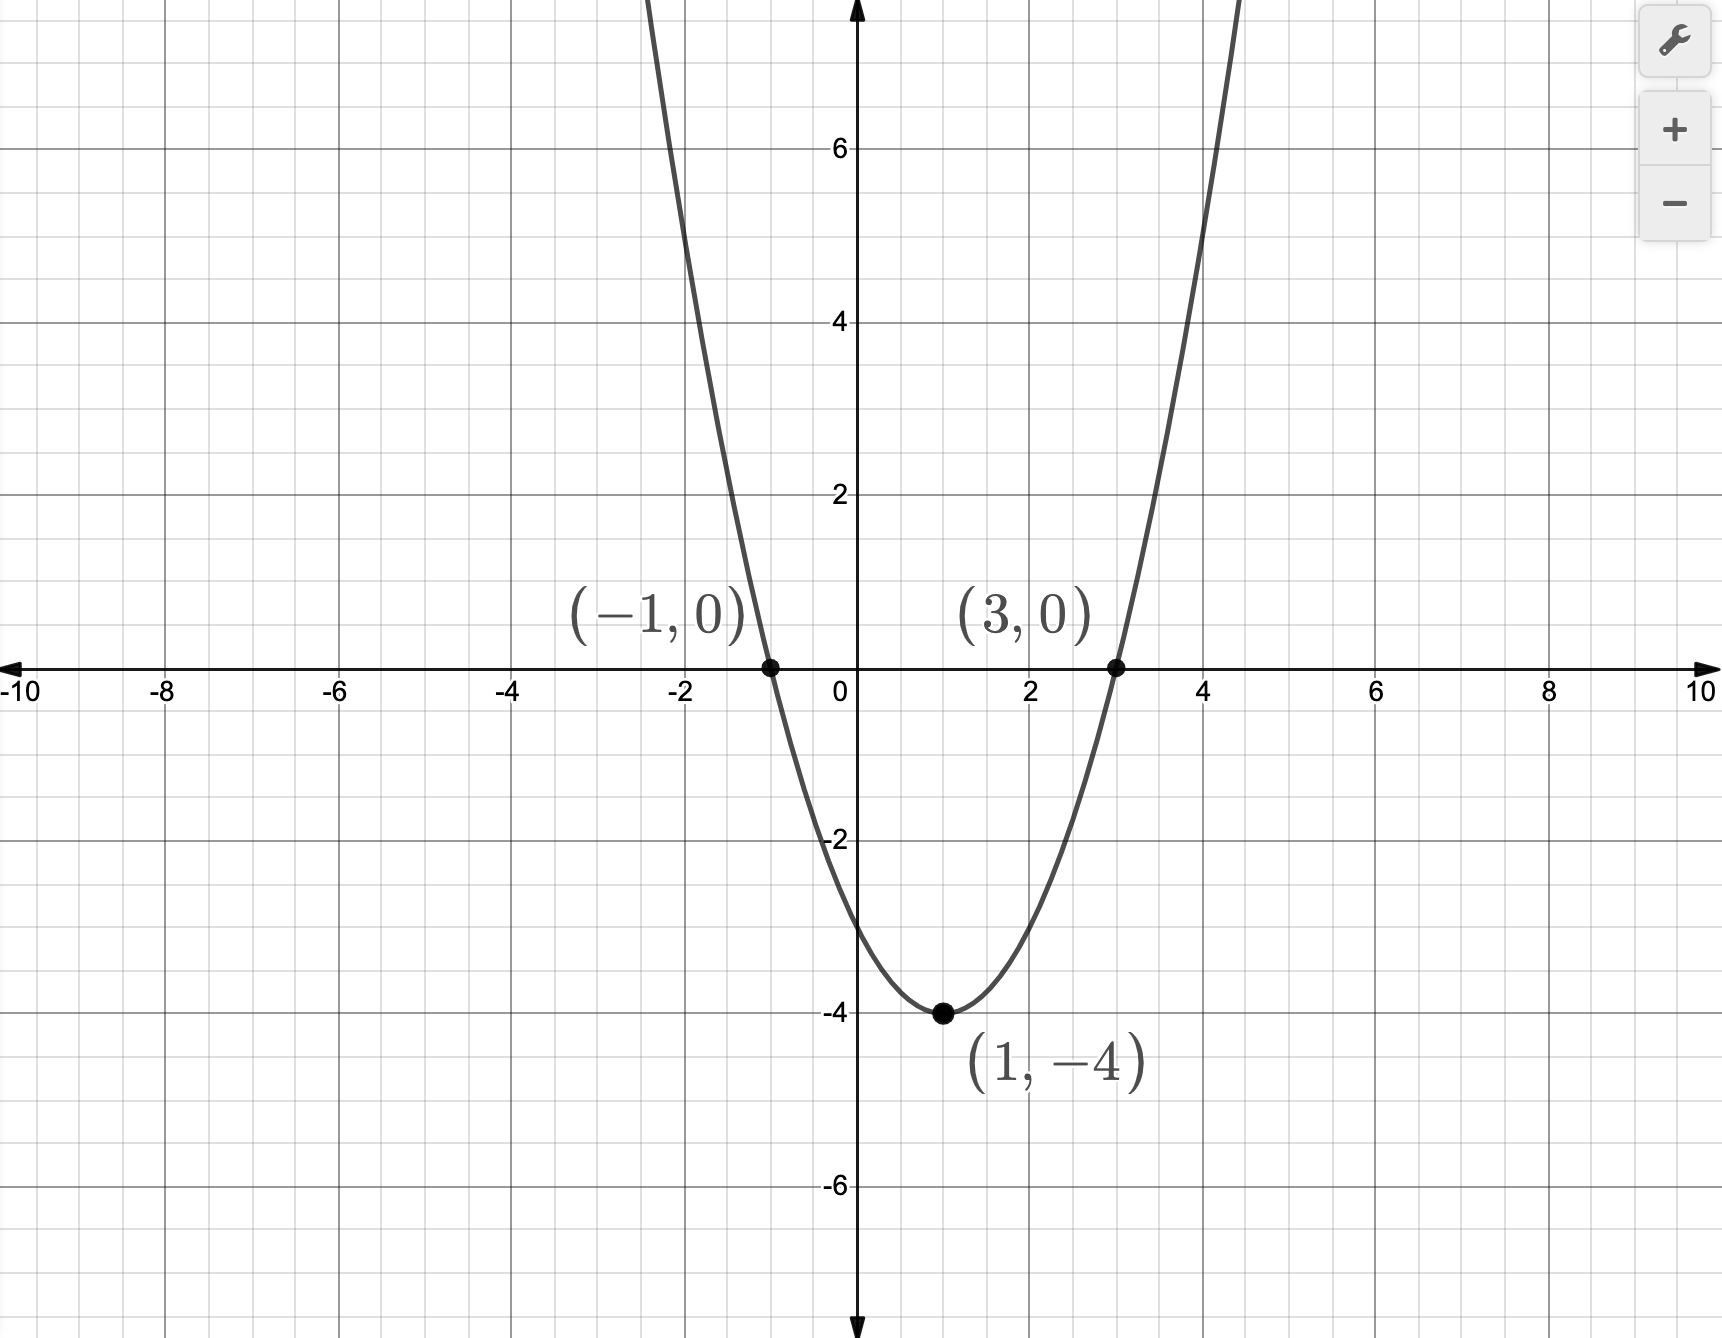
\includegraphics[scale=0.2]{4_1_025.png}
			\end{center}
		\end{figure}
	\end{enumerate}
\end{frame}

\begin{frame}
	\frametitle{Example (cont.)}
		\begin{enumerate}
			\item[]<1->find the zeros of $f(x)$:
			\item[]<2-> \textsc{Solution:} $x=-1, 3$;
			\item[]<3->the $x-$intercepts:
			\item[]<4->\textsc{Solution:} $x=-1, 3$;
			\item[]<5->the $y-$intercept:
			\item[]<6->\textsc{Solution:} $y=-3$;
			\item[]<7->the minimum:
			\item[]<8->\textsc{Solution:} $y=-4$;
			\item[]<9->the maximum:
			\item[]<10->\textsc{Solution:} $\infty$;
			\item[]<11->the domain:
			\item[]<12->\textsc{Solution:} $(-\infty, \infty)$;
			\item[]<13->the range:
			\item[]<14->\textsc{Solution:} $[-4, \infty)$.
		\end{enumerate}
\end{frame}

\begin{frame}
	\frametitle{Example}
	\begin{enumerate}
		\item[]<1-> Given
		\[
			g(x)=x^{3}+2x^{2}-11x-12=(x+4)(x+1)(x-3),
		\]
		\item[]<2->
		\begin{figure}
			\begin{center}
				\caption{$g(x)=x^{3}+2x^{2}-11x-12$}
				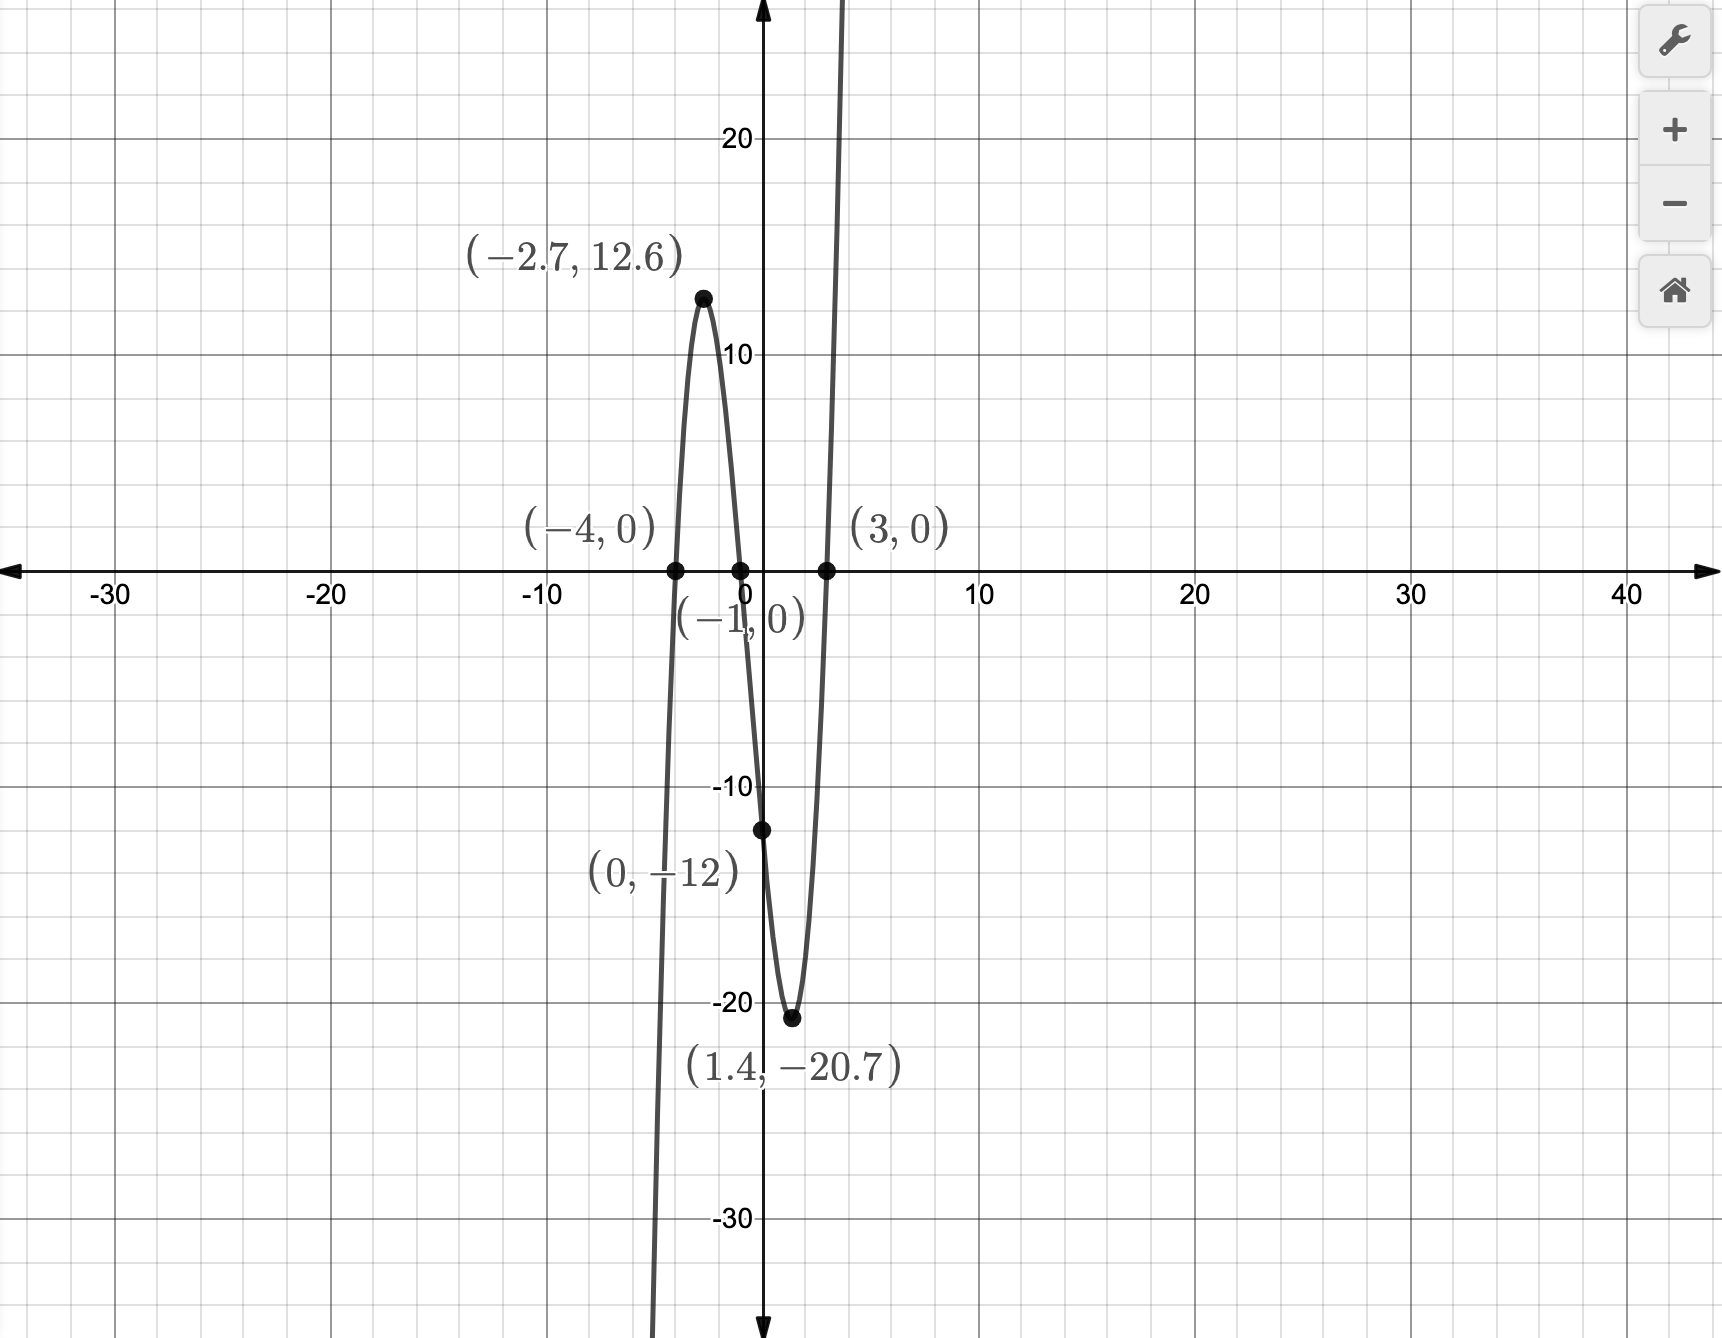
\includegraphics[scale=0.2]{4_1_050.png}
			\end{center}
		\end{figure}
	\end{enumerate}
\end{frame}

\begin{frame}
	\frametitle{Example (cont.)}
		\begin{enumerate}
			\item[]<1->find the zeros of $g(x)$:
			\item[]<2-> \textsc{Solution:} $x=-4, -1, 3$;
			\item[]<3->the $x-$intercepts:
			\item[]<4->\textsc{Solution:} $x=-4, -1, 3$;
			\item[]<5->the $y-$intercept:
			\item[]<6->\textsc{Solution:} $y=-12$;
			\item[]<7->the minimum:
			\item[]<8->\textsc{Solution:} $-\infty$;
			\item[]<9->the maximum:
			\item[]<10->\textsc{Solution:} $\infty$;
			\item[]<11->the domain:
			\item[]<12->\textsc{Solution:} $(-\infty, \infty)$;
			\item[]<13->the range:
			\item[]<14->\textsc{Solution:} $(-\infty, \infty)$.
		\end{enumerate}
\end{frame}

\begin{frame}
	\frametitle{Examples of Polynomial Functions}
	\begin{enumerate}
		\item[]<1->
		\begin{figure}
			\begin{center}
				\caption{Polynomial Functions}
				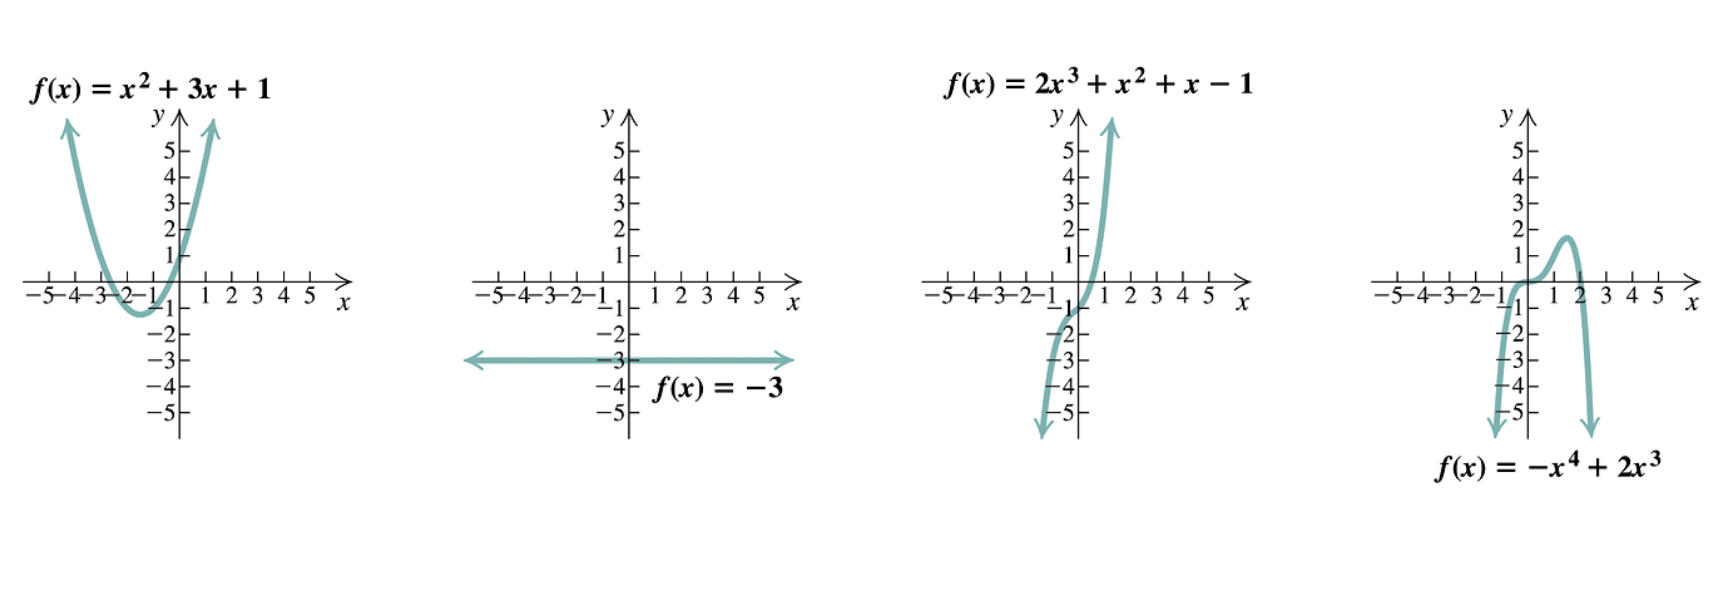
\includegraphics[scale=0.35]{4_1_1.png}
			\end{center}
		\end{figure}
	\end{enumerate}
\end{frame}

\begin{frame}
	\frametitle{Examples of Nonpolynomial Functions}
	\begin{enumerate}
		\item[]<1->
		\begin{figure}
			\begin{center}
				\caption{Nonpolynomial Functions}
				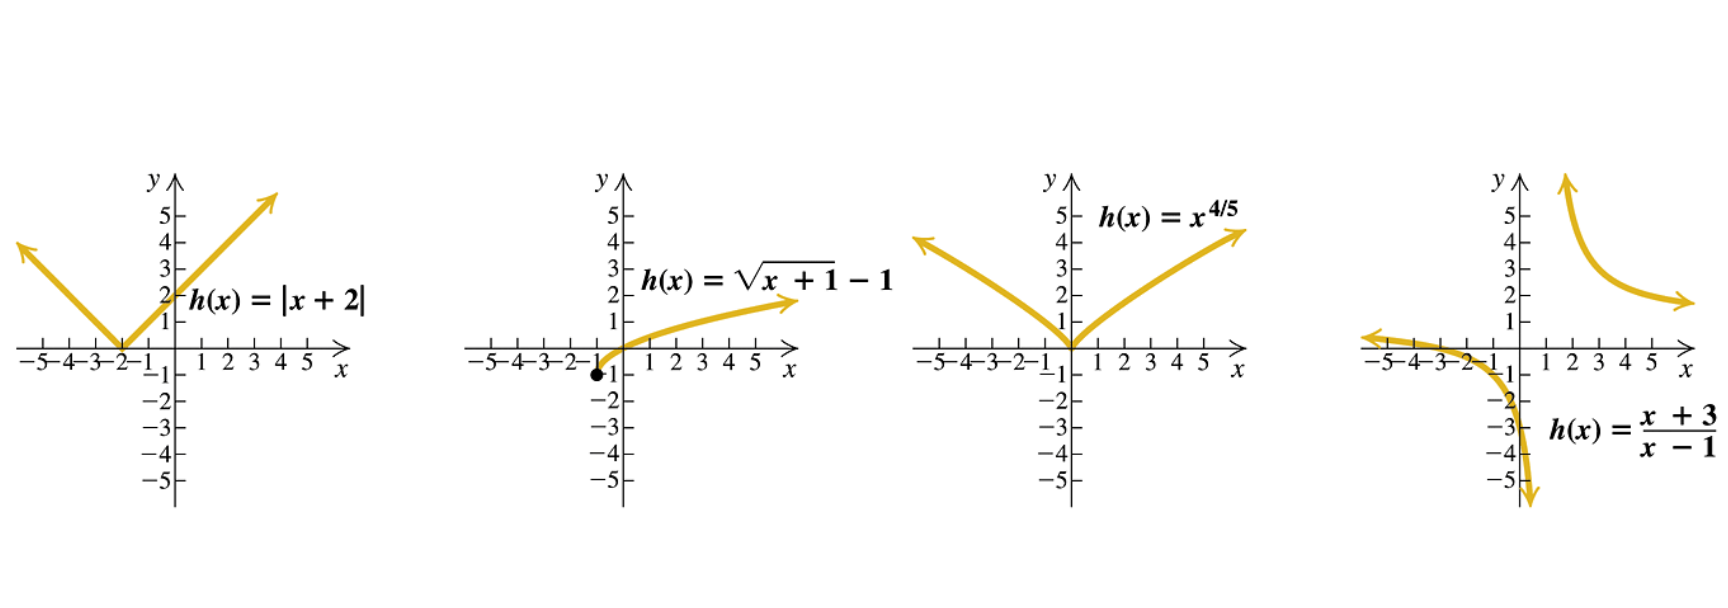
\includegraphics[scale=0.35]{4_1_2.png}
			\end{center}
		\end{figure}
	\end{enumerate}
\end{frame}

\begin{frame}
  \frametitle{Polynomial Functions}
  \begin{enumerate}
    \item[]<1->The graph of a polynomial function is \emph{continuous};  that is, it has no holes or breaks.
    \item[]<2->It is also smooth;  there are no ''sharp" corners.
    \item[]<3->Furthermore, the domain of a polynomial function is the set of all real numbers.
  \end{enumerate}
\end{frame}

\begin{frame}
  \frametitle{The Leading--Term Test}
  \begin{enumerate}
    \item[]<1->If $a_{n}x^{n}$ is the leading term of a polynomial function,
    \item[]<2->then the behavior of the graph as $x \rightarrow \infty$ or as $x \rightarrow -\infty$
    \item[]<3->can be described in one of the four following ways.
    \item[]<4->
    \begin{figure}
			\begin{center}
				\caption{}
				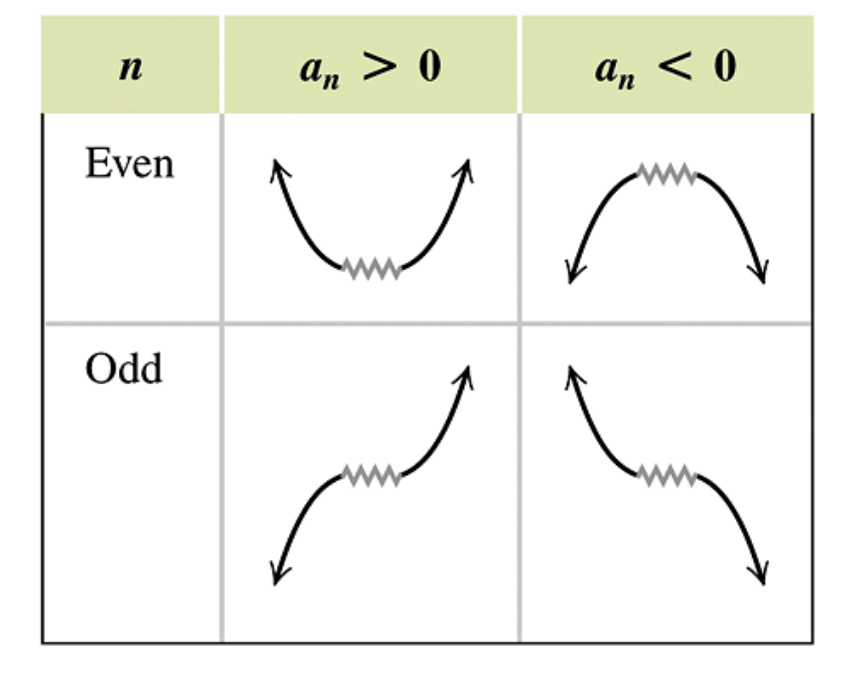
\includegraphics[scale=0.35]{4_1_3.png}
			\end{center}
		\end{figure}
  \end{enumerate}
\end{frame}

\begin{frame}
  \frametitle{Example}
  \begin{enumerate}
    \item[]<1->Using the leading term test, match each of the following functions with
    one of the graphs \textbf{A}--\textbf{D} that follow.
    \item[]<2->
    \begin{figure}
      \begin{center}
        \caption{}
        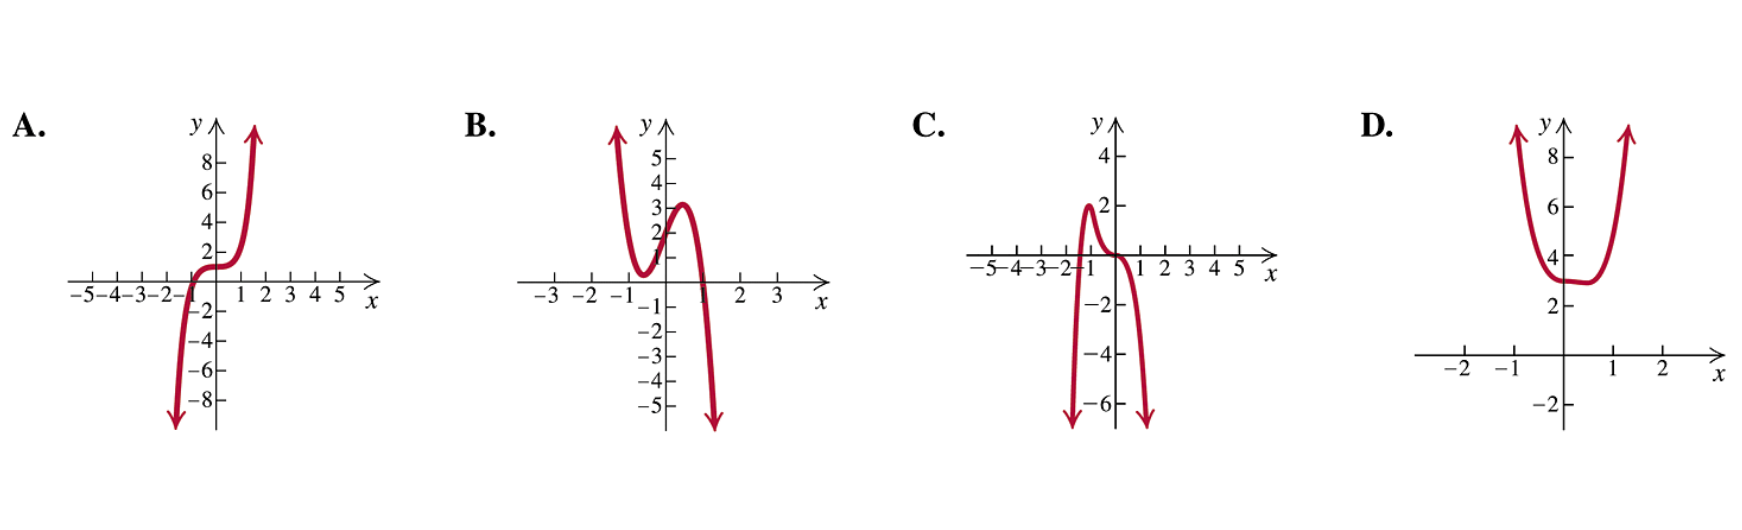
\includegraphics[scale=0.35]{4_1_4.png}
      \end{center}
    \end{figure}
  \end{enumerate}
\end{frame}

\begin{frame}
  \frametitle{Example (cont.)}
    \begin{enumerate}
      \item[]<1-> a. $f(x)=3x^{4}-2x^{3}+3$.
      \item[]<2-> \textsc{Solution:} \textbf{D}
      \item[]<3-> b. $f(x)=-5x^{3}-x^{2}+4x+2$
      \item[]<4-> \textsc{Solution:} \textbf{B}
      \item[]<5-> c. $f(x)=x^{5}+\frac{1}{4}x+1$
      \item[]<6-> \textsc{Solution:} \textbf{A}
      \item[]<7-> d. $f(x)=-x^{6}+x^{5}-4x^{3}$
      \item[]<8-> \textsc{Solution:} \textbf{C}
    \end{enumerate}
\end{frame}

\begin{frame}
  \frametitle{Example}
  \begin{enumerate}
    \item[]<1->Describe the end behavior of the graph of the following functions.
    \item[]<2->($1$) $f(x)=-x^{6}+\frac{3}{4}x^{4}$
    \item[]<3->\textsc{Solution:} $\frac{3}{4}x^{4}$ is the leading term. So $f(x) \rightarrow -\infty$ as $x \rightarrow -\infty$ and as $x \rightarrow \infty$.
    \item[]<4->($2$) $f(x)=3-\frac{1}{10}x+x^{5}$
    \item[]<5->\textsc{Solution:} $x^{5}$ is the leading term. So $f(x) \rightarrow -\infty$ as $x \rightarrow -\infty$, and $f(x) \rightarrow \infty$ as $x \rightarrow \infty$.
  \end{enumerate}
\end{frame}

\begin{frame}
  \frametitle{Example (cont.)}
  \begin{enumerate}
    \item[]<1->($3$) $f(x)=2x^{4}-x^{2}+1$
    \item[]<2->\textsc{Solution:} $2x^{4}$ is the leading term.  So $f(x) \rightarrow \infty$ as $x \rightarrow \infty$ and as $x \rightarrow -\infty$.
    \item[]<3->($4$) $f(x)=x^{2}-x^{3}-2x+4$.
    \item[]<4-> \textsc{Solution:} $-x^{3}$ is the leading term.  So $f(x) \rightarrow \infty$ as $x \rightarrow -\infty$, and $f(x) \rightarrow -\infty$ as $x \rightarrow \infty$.
  \end{enumerate}
\end{frame}

\begin{frame}
	\frametitle{Example}
	\begin{enumerate}
		\item[]<1-> Choose the end behavior diagram that best describes the function $f(x)=-3.9x^{4}+x^{6}+0.1x^{7}$.
		\item[]<2->
    \begin{figure}
      \begin{center}
        \caption{}
        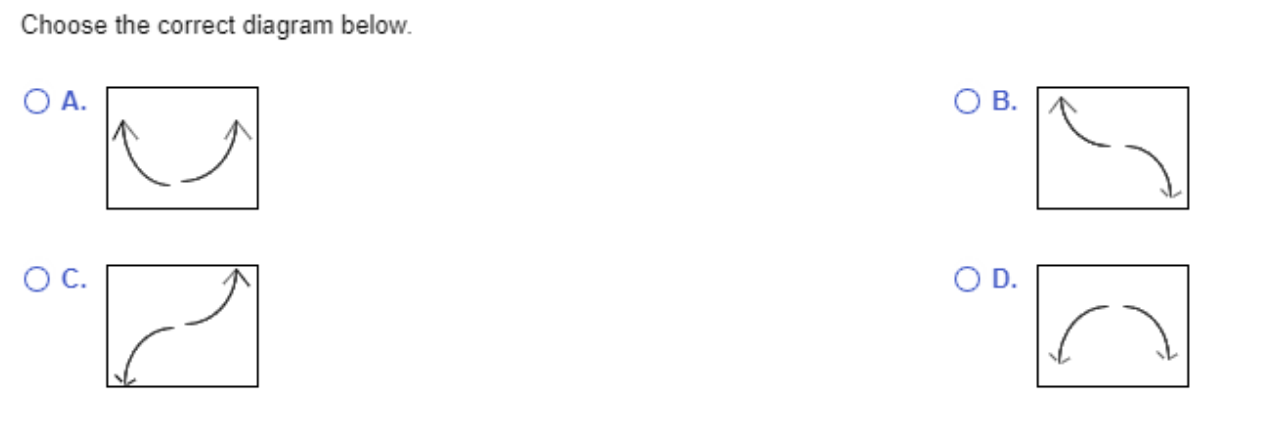
\includegraphics[scale=0.35]{4_1_5.png}
      \end{center}
      \item[]<3-> \textsc{Solution:} $f(x) \approx x^{7} \Rightarrow $C.
    \end{figure}
	\end{enumerate}
\end{frame}

\begin{frame}
	\frametitle{Example}
	\begin{enumerate}
		\item[]<1-> Choose the end behavior diagram that best describes the function $f(x)=5+\frac{1}{5}x^{4}-\frac{1}{2}x^{3}$.
		\item[]<2->
    \begin{figure}
      \begin{center}
        \caption{}
        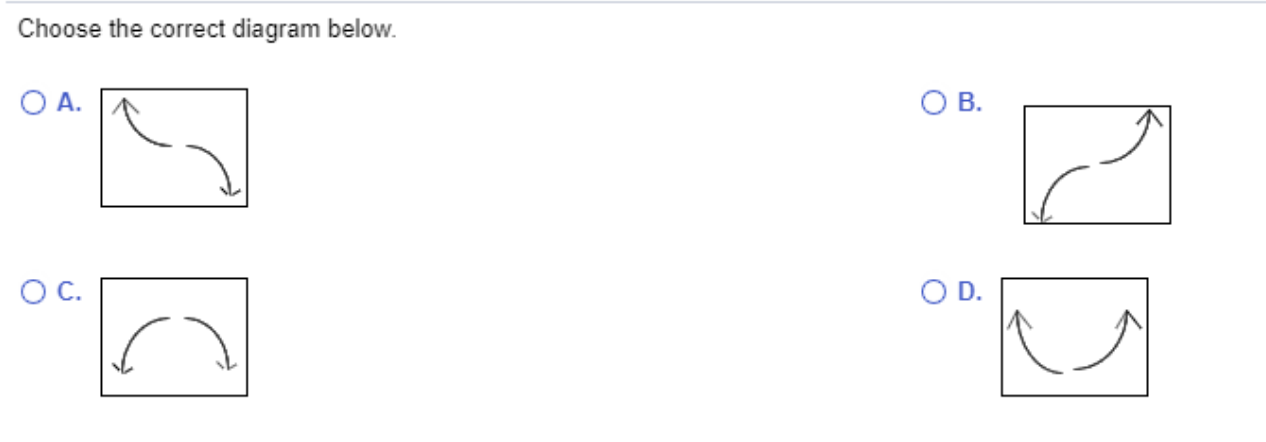
\includegraphics[scale=0.35]{4_1_6.png}
      \end{center}
      \item[]<3-> \textsc{Solution:} $f(x) \approx x^{4} \Rightarrow $D.
    \end{figure}
	\end{enumerate}
\end{frame}

\begin{frame}
	\frametitle{Example}
	\begin{enumerate}
		\item[]<1-> Use the leading term test to match the function $f(x)=x^{5}+\frac{1}{14}x-3$ with one of the given graphs.
		\item[]<2->
    \begin{figure}
      \begin{center}
        \caption{}
        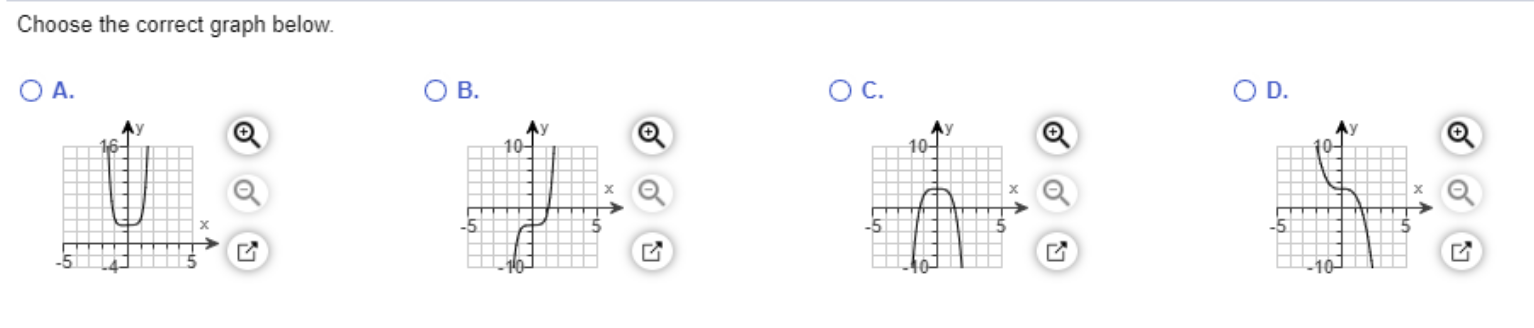
\includegraphics[scale=0.375]{4_1_7.png}
      \end{center}
      \item[]<3-> \textsc{Solution:} $f(x) \approx x^{5} \Rightarrow $B.
    \end{figure}
	\end{enumerate}
\end{frame}

\begin{frame}
	\frametitle{Finding Zeros of Polynomial Functions}
	\begin{enumerate}
		\item[]<1->If $c$ is a real zero of a function (that is, $f(c)=0$),
		\item[]<2->then $(c,0)$ is an $x-$intercept of the graph of the function.
	\end{enumerate}
\end{frame}

\begin{frame}
	\frametitle{Even and Odd Multiplicity}
	\begin{enumerate}
		\item[]<1->If $(x-c)^{k}, k \geq 1$, is a factor of a polynomial function $P(x)$ and $(x-c)^{k+1}$ is not a factor and:
		\item[]<2-> (i) $k$ is odd, then the graph crosses the $x-$axis at $(c,0)$;
		\item[]<3-> (ii) $k$ is even, then the graph is tangent to the $x-$axis at $(c,0)$.
	\end{enumerate}
\end{frame}

\begin{frame}
  \frametitle{Example}
    \begin{enumerate}
      \item[]<1->Use substitution to determine whether $3$ is a zero of
      \item[]<2-> \[ (a)~f(x)=x^{3}-10x^{2}+17x+12. \]
      \item[]<3-> \textsc{Solution:}
      \item[]<4-> \[ f(3)=3^{3}-10(3^{2})+17(3)+12 \]
      \item[]<5-> \[ \Rightarrow f(3)=27-90+51+12=0 \]
      \item[]<6-> Thus $3$ is a zero of $f(x)$.
    \end{enumerate}
\end{frame}

\begin{frame}
  \frametitle{Example}
    \begin{enumerate}
      \item[]<1->Use substitution to determine whether $3$ is a zero of
      \item[]<2-> \[ (b)~f(x)=x^{4}-5x^{3}-2x-15. \]
      \item[]<3-> \textsc{Solution:}
      \item[]<4-> \[ f(3)=3^{4}-5(3^{2})-2(3)-15 \]
      \item[]<5-> \[ \Rightarrow f(3)=-75 \]
      \item[]<6-> Thus $3$ is \emph{not} a zero of $f(x)$.
    \end{enumerate}
\end{frame}

\begin{frame}
  \frametitle{Example}
    \begin{enumerate}
      \item[]<1-> Find the zeros of $f(x)=5(x-2)(x-2)(x-2)(x+1)$ and determine the multiplicity of each.
      \item[]<2-> \textsc{Solution:}
      \item[]<3-> Rewrite $f(x)=5(x-2)^{3}(x+1)$.
      \item[]<4-> $x=2$ is a zero of $f(x)$
      \item[]<5-> with a multiplicity of $3$.
      \item[]<6-> $x=-1$ is a zero of $f(x)$
      \item[]<7-> with a multiplicity of $1$
    \end{enumerate}
\end{frame}

\begin{frame}
  \frametitle{Example}
    \begin{enumerate}
      \item[]<1-> Find the zeros of $f(x)=-(x-1)^{2}(x+2)^{2}$ and determine the multiplicity of each.
      \item[]<2-> \textsc{Solution:}
      \item[]<3-> $x=1$ is a zero of $f(x)$
      \item[]<4-> with a multiplicity of $2$.
      \item[]<5-> $x=-2$ is a zero of $f(x)$
      \item[]<6-> with a multiplicity of $2$
    \end{enumerate}
\end{frame}

\begin{frame}
  \frametitle{Example}
    \begin{enumerate}
      \item[]<1-> Find the zeros of $f(x)=x^{3}-2x^{2}-9x+18$ and determine the multiplicity of each.
      \item[]<2-> \textsc{Solution:}
      \item[]<3-> Factor $f(x)=x^{2}(x-2)-9(x-2)=(x-2)(x-3)(x+3)$.
      \item[]<4-> $x=2$ is a zero of $f(x)$
      \item[]<5-> with a multiplicity of $1$.
      \item[]<6-> $x=3$ is a zero of $f(x)$
      \item[]<7-> with a multiplicity of $1$
      \item[]<8-> $x=-3$ is a zero of $f(x)$
      \item[]<9-> with a multiplicity of $1$.
    \end{enumerate}
\end{frame}

\begin{frame}
  \frametitle{Example}
    \begin{enumerate}
      \item[]<1-> Find the zeros of $f(x)=2x^{3}-x^{2}-14x+7$ and determine the multiplicity of each.
      \item[]<2-> \textsc{Solution:}
      \item[]<3-> Factor $f(x)=x^{2}(2x-1)-7(2x-1)=(2x-1)(x^{2}-7)$.
      \item[]<4-> $x=\frac{1}{2}$ is a zero of $f(x)$
      \item[]<5-> with a multiplicity of $1$.
      \item[]<6-> $x=\sqrt{7}$ is a zero of $f(x)$
      \item[]<7-> with a multiplicity of $1$
      \item[]<8-> $x=-\sqrt{7}$ is a zero of $f(x)$
      \item[]<9-> with a multiplicity of $1$.
    \end{enumerate}
\end{frame}

\begin{frame}
  \frametitle{Example}
    \begin{enumerate}
      \item[]<1-> Find the zeros of $f(x)=x^{3}-x^{2}$ and determine the multiplicity of each.
      \item[]<2-> \textsc{Solution:}
      \item[]<3-> Factor $f(x)=x^{2}(x-1)$.
      \item[]<4-> $x=1$ is a zero of $f(x)$
      \item[]<5-> with a multiplicity of $1$.
      \item[]<6-> $x=0$ is a zero of $f(x)$
      \item[]<7-> with a multiplicity of $2$
    \end{enumerate}
\end{frame}

\begin{frame}
  \frametitle{Example}
    \begin{enumerate}
      \item[]<1-> Find the zeros of $f(x)=(x+1)^{4}(x-3)$ and determine the multiplicity of each.
      \item[]<2-> \textsc{Solution:}
      \item[]<3-> $x=-1$ is a zero of $f(x)$
      \item[]<4-> with a multiplicity of $4$.
      \item[]<5-> $x=3$ is a zero of $f(x)$
      \item[]<6-> with a multiplicity of $1$
    \end{enumerate}
\end{frame}

\begin{frame}
  \frametitle{Example}
  \begin{enumerate}
    \item[]<1->Determine whether the following statement is true or false.
    \item[]<2->``If $P(x)=(x-7)^{7}(x+5)^{2}$, then the graph of the polynomial function $y=P(x)$ is tangent to the $x-$axis at $(-5,0)$. "
    \item[]<3->\textsc{Solution:}
    \item[]<4-> $P(x)$ has a zero at $x=-5$.
    \item[]<5-> This zero has a multiplicty of $2$, an even number.
    \item[]<6-> Thus $P(x)$ is tangent to the $x-$axis at $(-5,0)$
    \item[]<7-> The statement is true (Statement B).
  \end{enumerate}
\end{frame}

\begin{frame}
  \frametitle{Example}
  \begin{enumerate}
    \item[]<1->Find the correct end behavior diagram for the given polynomial function.
    \item[]<2-> \[ f(x)=-2.76x^{4}-x^{3}+x^{2}-2x+1. \]
    \item[]<3-> \textsc{Solution:}
    \item[]<4-> $f(x) \sim -x^{4}$.
    \item[]<5->Choose D.  
  \end{enumerate}
\end{frame}


\end{document}
